\documentclass[12pt, a4paper]{article}
\usepackage[a4paper, top=2cm, bottom=3cm, left=2cm, right=2cm]{geometry}
\usepackage[export]{adjustbox}
\usepackage{graphicx}
\usepackage{mathtools}
\usepackage{hyperref}
\usepackage{amsmath}
\usepackage{amsfonts}
\usepackage{amssymb}
\usepackage[version=4]{mhchem}
\usepackage{stmaryrd}
\usepackage{polyglossia}
\usepackage{fontspec}
\usepackage{ucharclasses}
\usepackage{fancyhdr}
\usepackage{wrapfig}
\usepackage{subcaption}
\usepackage{relsize}
\usepackage{framed}
\usepackage{changepage}
\usepackage{tabularray}
\usepackage{etoolbox}
\usepackage{xstring}
\usepackage{pstricks-add}
\usepackage{tikz}
\usepackage{empheq}
\usepackage{tcolorbox}
\usepackage[european,s traightvoltages, americanresistor, americaninductors]{circuitikz}
\usepackage{pgfplots}
\usepackage{tikz-3dplot}

\usetikzlibrary{
	angles,
	arrows.meta,
	positioning,
	arrows,
	backgrounds,
	calc,
	decorations,
	decorations.markings,
	decorations.pathmorphing,
	fit,
	shapes.arrows,
	shapes.callouts,
	shapes.geometric,
	shapes.misc,
	snakes,
	quotes
}
\pgfplotsset{compat=1.18}
\hypersetup{colorlinks=true, linkcolor=blue, filecolor=magenta, urlcolor=cyan,}
\urlstyle{same}

\setmainlanguage{english}
\setotherlanguages{norwegian, arabic}
\newfontfamily\arabicfont{Noto Naskh Arabic}
% \newfontfamily\lgcfont{CMU Serif}

%%%%%%%%%% Fancy header %%%%%%%%%
\pagestyle{fancy}
\fancyhead[C]{}
\fancyfoot[C]{\medskip\thepage}
\renewcommand{\footrulewidth}{.4pt}
\renewcommand{\headrulewidth}{0pt}

\setlength{\headheight}{14.49998pt}
\addtolength{\topmargin}{-2.49998pt}

\newcommand{\figwidth}{8cm}
\newcommand{\floatfigwidth}{5cm}


%%%%%%%%%% Formatters & Layout %%%%%%%%%
\newcommand{\uprimary}[1]{
	\section*{\center \Huge \underline{#1}}
	\addcontentsline{toc}{section}{\protect\numberline{}#1}
}
\newcommand{\usecondary}[1]{
	\section*{\center \LARGE \underline{#1}}
	\addcontentsline{toc}{section}{\protect\numberline{}#1}
}
\newcommand{\usection}[1]{
	\section*{\LARGE #1}
	\addcontentsline{toc}{subsection}{\protect\numberline{}#1}
}
\newcommand{\usubsection}[1]{
	\section*{\Large #1}
	\addcontentsline{toc}{subsection}{\protect\numberline{}#1}
}
\newcommand{\ussubsection}[1]{
	\section*{\large #1}
	\addcontentsline{toc}{subsection}{\protect\numberline{}#1}
}
\newcommand{\ans}{\bigskip\underline{\textbf{Answer}}}
\newcommand{\ques}[1]{\noparindent\textbf{#1}\doparindent}
\newcommand{\rfloatingimg}[1]{
	\begin{wrapfigure}{r}{\floatfigwidth}
		\includegraphics[max width=\floatfigwidth]{#1}
	\end{wrapfigure}
}
\newcommand{\indentbox}[2]{
	\begin{adjustwidth}{#1}{0pt}
		#2
	\end{adjustwidth}
}
\newcommand{\qa}[3]{
	\noparindent
	\textbf{#1 #2}
	\indentbox{.76cm}{
		\ans
		#3
	}
	\vspace{.75cm}
}
\newcommand{\noskipqa}[2]{
	\noparindent
	\textbf{#1}
	\indentbox{.76cm}{
		\ans
		#2
	}
}
\newcommand{\eqnleft}[1]{
	\begin{flalign*}
		 & #1 &  &
	\end{flalign*}
}
\newcommand{\fullwidthimg}[1]{
	\begin{center}
		\includegraphics[max width=\textwidth]{#1}
	\end{center}
}
\newcommand{\uheading}[2]{
	\uprimary{Module - #1}
	\vspace{-.7cm}
	\usecondary{#2}
}

\newcommand{\note}[1]{
	\begin{tcolorbox}[colframe=green!40!black, colback=green!5!white, title={\textbf{Note}}]
	#1
	\end{tcolorbox}
}


%%%%%%%%%% general constants/symbols %%%%%%%%%
\newcommand\longUparrow{\mathrel{\scalebox{1}[2]{$\uparrow$}}}
\DeclareRobustCommand{\rchi}{{\mathpalette\irchi\relax}}
\newcommand{\irchi}[2]{\raisebox{\depth}{$#1\chi$}}
\newcommand{\term}[1]{\underline{\textbf{#1}}}
\newcommand{\amstr}{\mathring{\textrm{A}}}
\newcommand{\h}{6.626 \times 10^{-34}}
\newcommand{\kB}{1.38 \times 10^{-23}}
\newcommand{\lc}{3 \times 10^{8}}
\newcommand{\uunit}[1]{\mathrm{~#1}}

%%%%%%%%%% Format constants %%%%%%%%%
\newcommand{\doparindent}{\setlength\parindent{.5cm}}
\newcommand{\noparindent}{\setlength\parindent{0pt}}
\graphicspath{ {../images/} }
\NewDocumentCommand{\multiskip}{m}{%
	\begingroup
	\newcount\i  % Define a new counter \i
	\i=0         % Initialize the counter
	\loop
	\ifnum\i<#1
	\bigskip  % Add \bigskip
	\advance\i by 1  % Increment the counter
	\repeat
	\endgroup
}

\newcommand{\termlist}[1]{
	\begin{tcolorbox}[colback=blue!10!white, colframe=blue!50!black, title={Some terms}]
		#1
	\end{tcolorbox}
}


%%%%% dev fx
% startx, starty, endx, endy
\newcommand{\dottedgrid}[4]{
	\draw[thin, dotted] (#1, #2) grid (#3,#4);
	\foreach \i in {#1,...,#3} \node at (\i,-2ex) {\i};
	\foreach \i in {#2,...,#4} \node at (-2ex,\i) {\i};
}
\newcommand{\smallmidarrow}[2]{\tikz \draw[arrows = {-Straight Barb[scale=.8]}, line width=#1] (0,0) -- +(#2,0);}
\newcommand{\midarrow}[2]{\tikz \draw[arrows = {-Straight Barb[scale=1.1]}, line width=#1] (0,0) -- +(#2,0);}

\DefTblrTemplate{caption-tag}{default}{}
\DefTblrTemplate{caption-sep}{default}{}
\DefTblrTemplate{caption-text}{default}{}
\DefTblrTemplate{contfoot-text}{default}{}
\DefTblrTemplate{conthead-text}{default}{}

\usepackage{tikz}
\usepackage{listofitems}
\usepackage{xargs}
\usepackage{fp}
\usetikzlibrary{3d,calc,patterns,quotes,angles,perspective}

\newcommandx{\shadedPlane}[6][5=blue, 6=0.8]{
	\readlist\a{#1}%
	\readlist\b{#2}%
	\readlist\c{#3}%
	\readlist\d{#4}%
	\coordinate (P1) at (\a[1], \a[2], \a[3]);
	\coordinate (P2) at (\b[1], \b[2], \b[3]);
	\coordinate (P3) at (\c[1], \c[2], \c[3]);
	\coordinate (P4) at (\d[1], \d[2], \d[3]);
	\fill[pattern=north east lines, pattern color=#5, opacity=#6]
	(P1) -- (P2) -- (P3) -- (P4)-- cycle;
	\draw[thick, color=#5, opacity=#6]
	(P1) -- (P2) -- (P3) -- (P4) -- cycle;
}

\newcommandx{\axes}[2][1=1, 2=1.3]{
	\FPeval\axside{#1 * #2}
	\draw[->, red] (0,0,0) -- (\axside,0,0) node[anchor=north east] {$x$};
	\draw[->, green] (0,0,0) -- (0,\axside,0) node[anchor=north west] {$y$};
	\draw[->, blue] (0,0,0) -- (0,0,\axside) node[anchor=south] {$z$};
}
\newcommandx{\wirecube}[2][2=1pt]{
	% vertices of the cube & plane
	\coordinate (A) at (0,0,0);
	\coordinate (B) at (#1,0,0);
	\coordinate (C) at (#1,#1,0);
	\coordinate (D) at (0,#1,0);
	\coordinate (E) at (0,0,#1);
	\coordinate (F) at (#1,0,#1);
	\coordinate (G) at (#1,#1,#1);
	\coordinate (H) at (0,#1,#1);

	% Draw the edges of the cube
	\draw[thick] (A) -- (B) -- (C) -- (D) -- cycle;
	\draw[thick] (E) -- (F) -- (G) -- (H) -- cycle;
	\draw[thick] (A) -- (E);
	\draw[thick] (B) -- (F);
	\draw[thick] (C) -- (G);
	\draw[thick] (D) -- (H);

	% Add points to illustrate vertices
	\foreach \i in {(A), (B), (C), (D), (E), (F), (G), (H)} {
			\filldraw[black] \i circle (#2);
		}
}

\newcommand{\wirecubewithlabels}[2]{
	\wirecube{#1}[#2]

	% Label the side lengths

	\coordinate (A) at (0,0,0);
	\coordinate (B) at (#1,0,0);
	\coordinate (D) at (0,#1,0);
	\coordinate (E) at (0,0,#1);

	\node at ($(A)!0.8!(B)$) [above] {$\vec{a}$};
	\node at ($(A)!0.7!(D)$) [above right] {$\vec{b}$};
	\node at ($(A)!0.7!(E)$) [above] {$\vec{c}$};
	\draw[thick, ->] (A) -- (B);
	\draw[thick, ->] (A) -- (D);
	\draw[thick, ->] (A) -- (E);
	\pic [blue,draw,angle radius=0.25cm] {angle=B--A--E};
	\pic [green,draw,angle radius=0.25cm] {angle=D--A--B};
	\pic [red,draw,angle radius=0.25cm] {angle=D--A--E};

	\node[color=blue, scale=.8] at (.4,0.4,0) {$\gamma$};
	\node[color=green, scale=.8] at (.7,0,.7) {$\beta$};
	\node[color=red, scale=.8] at (-0.3,0.3,0.3) {$\alpha$};
}

\newcommand{\smallmidarrow}[2]{\tikz \draw[arrows = {-Straight Barb[scale=.8]}, line width=#1] (0,0) -- +(#2,0);}
\newcommand{\midarrow}[2]{\tikz \draw[arrows = {-Straight Barb[scale=1.1]}, line width=#1] (0,0) -- +(#2,0);}
\newcommand{\millerDiagramQuad}[6]{
	\begin{tikzpicture}[
			scale=#6,
			x={(-.45cm, -.4cm)},
			y={(1cm, 0cm)},
			z={(0cm, 1cm)}
		]
		\axes[#5]
		\shadedPlane{#1}{#2}{#3}{#4}

		\wirecube{#5}[0pt]

	\end{tikzpicture}
}

\newcommand{\millerDiagram}[5]{
	\millerDiagramQuad{#1}{#2}{#3}{#3}{#4}{#5}
}

\newcommand{\doubleCylinder}[3]{
	\draw (0,0) ellipse (#1 and #1*2);
	\draw (0,#1*2) -- ++(#3, 0);
	\draw (0,-#1*2) -- ++(#3, 0);

	\draw (0,0) ellipse (#2 and #2*2);
	\draw (0,#2*2) -- ++(#3, 0);
	\draw (0,-#2*2) -- ++(#3, 0);
}

% x,y, r, y-scalar, x-length, y-shear, color
\newcommand{\cylinder}[7]{
	\begin{scope}[shift={(#1, #2)}]
		\draw[fill=#7, draw=black] (#5, #4*#3+#6) arc (90:-80:#3 and #4*#3) -- ++(-#5, -#6) arc (-80:90:#3 and #4*#3) -- cycle;
		\draw[fill=#7, draw=black] (0, 0) ellipse (#3 and #4*#3);
	\end{scope}
}


\begin{document}
2.
Partial Differentiation

Partial Differentiation
Let $z=f(x, y)$, be a function of $x, y$. Then partial derivative wet. $x$ is denoted by: $\frac{\partial x}{\partial x} \cdot \frac{\partial z}{\partial x}$ It means differentiating $\approx z$ wit $x$ while keeping $y$ as constant.
Similarly $\frac{\partial z}{\partial y}$ represents partial derivative of $z$ wot $y$ keeping $x$ constant
In all the cases:
$$
\frac{\partial z}{\partial x} \cdot \frac{\partial z}{\partial y} \equiv \frac{\partial z^2}{\partial x \partial y}=\frac{\partial}{\partial y} \cdot \frac{\partial z}{\partial x} \equiv \frac{\partial z^2}{\partial y y \partial x}
$$
1. Find $1^{17} d z^{\text {nd }}$ partial derivative of $z=x^3+y^3-3 a x y$
s.)
$$
\begin{array}{ll}
\frac{\partial z}{\partial x}=3 x^2-3 a y, \frac{\partial z^2}{\partial x^2}=6 x, & \frac{\partial \cdot \partial z^2}{\partial x \partial y}=3 a \\
\frac{\partial z}{\partial y}=3 y^2-3 a x, \frac{\partial z^2}{\partial y^2}=6 y, & \frac{\partial z^2}{\partial y \partial x}=3 a \\
\text { * here: } \frac{\partial z^2}{\partial x \partial y}=\frac{\partial z^2}{\partial y \partial x}
\end{array}
$$
2. If $v=\left(x^2+y^2+z^2\right)^{-1 / 2}$, find $\frac{\partial^2 v}{\partial x^2}+\frac{\partial^2 v}{\partial y^2}+\frac{\partial^2 v}{\partial z^2}$
A.
$$
\begin{aligned}
\frac{\partial^2 y}{\partial x^2}= & \frac{\partial v}{\partial x}=-\frac{1}{2}\left(x^2+y^2+z^2\right)^{-3 / 2} \cdot 2 x, \quad \frac{\partial x^2}{\partial / 2}=-z x \cdot\left(x^2\right. \\
& \frac{\partial v}{\partial y}=-\frac{1}{2}\left(x^2+y^2+z^2\right)^{-3 / 2} \cdot 2 y \\
& \frac{\partial v}{\partial z}=-\frac{1}{2}\left(x^2+y^2+z^2\right)^{-3 / 2} \cdot 2 z
\end{aligned}
$$

$\frac{\partial^{2} t}{\partial x^{2}}=-\left(x^{2}+y^{2}+z^{2}\right)^{-3 / 2}+x \cdot \frac{3}{2}\left(x^{2}+y^{2}+z^{2}\right)^{5 / 2} \times 2 x$

$=\frac{3 x^{2}}{\left(x^{2}+y^{2}+z^{2}\right)^{5 / 2}}-\frac{1}{\left(x^{2}+y^{2}+z^{2}\right)^{3 / 2}}$

$\frac{\partial^{2} v}{\partial y^{2}}=\frac{3 y^{2}}{\left(x^{2}+y^{2}+z^{2}\right)^{5 / 2}}-\frac{1}{\left(x^{2}+y^{2}+z^{2}\right)^{3 / 2}}$

$\frac{\partial^{2} v}{\partial z^{2}}=\frac{\partial z^{2}}{\left(x^{2}+y^{2}+z^{2}\right)^{5 / 2}}-\frac{1}{\left(x^{2}+y^{2}+z^{2}\right)^{3 / 2}}$

$\therefore \frac{\partial^{2} x}{\partial x^{2}}+\frac{\partial^{2} v}{\partial y^{2}}+\frac{\partial^{2} v}{\partial z^{2}}=\frac{3}{\left(x^{2}+y^{2}+z^{2}\right)^{7 /}}\left(\frac{x^{2}+y^{2}+z^{2}}{\left(x^{2}+y^{2}+z^{2}\right)}-1\right)$

\begin{itemize}
  \item If $u=x^{2} \tan ^{-1}(7 x)-y^{2} \tan ^{-1}\left(\frac{x}{y}\right)$ find $\frac{\partial^{2} u}{\partial x \partial y}$ and
\end{itemize}

show that $u_{x y}=u_{y x}$\\
A) $\frac{\partial u}{\partial y}=x^{2} \cdot \frac{1}{1+(y / x)^{2}} \frac{1}{x}-2 y \tan ^{-1}\left(\frac{x}{y}\right)-y^{2} \cdot \frac{1}{1+\left(\frac{x}{y}\right)^{2}} \cdot \frac{-1}{y^{2}}$

$$
=x^{2} \cdot \frac{x^{2}}{x^{2}+y^{2}} \frac{1}{x}+y^{2} \cdot \frac{y^{2}}{x^{2}+y^{2}} \frac{x}{y^{2}}-2 y \tan ^{-1}\left(\frac{x}{y}\right)
$$


\begin{equation*}
\frac{x^{3}}{x^{2}+y^{2}}+\frac{x y^{2}}{x^{2}+y^{2}}-2 y \tan ^{-1}\left(\frac{x}{y}\right)=x-2 y \tan ^{-1} \tag{x}
\end{equation*}


$\frac{\partial u}{\partial x \partial y}=\frac{\partial}{\partial x}\left(x-2 y \tan ^{-1}\left(\frac{x}{y}\right)\right)$

$=1-2 y \cdot \frac{1}{1+\left(\frac{x}{y}\right)^{2}} \cdot \frac{1}{y}=1-\frac{2 y^{2}}{x^{2}+y^{2}}=\frac{x^{2}-y^{2}}{x^{2}+y^{2}}$

$\frac{\partial u}{\partial x}=2 x \cdot \tan ^{-1}\left(\frac{y}{x}\right)+x^{2} \cdot \frac{1}{1+\left(\frac{y}{x}\right)^{2}} \times \frac{y}{x^{2}}-y^{2} \cdot \frac{1}{1+\frac{x^{2}}{y^{2}}} \cdot \frac{1}{y}$

$$
\begin{aligned}
& =2 x \tan ^{-1}\left(\frac{y}{x}\right)-\frac{y x^{2}}{x^{2}+y^{2}}-\frac{y^{3}}{x^{2}+y^{2}} \\
& =2 x \tan ^{-1}\left(\frac{y}{x}\right)-y
\end{aligned}
$$

$\frac{\partial u}{\partial y \partial x}=2 x \frac{1}{1+y^{2} x^{2}} \frac{1}{x} \phi-1$

$$
=\frac{2 x x^{2}}{x^{2}+y^{2}}-1 \Rightarrow \frac{x^{2}-y^{2}}{x^{2}+y^{2}}
$$

$\therefore \frac{\partial u}{\partial y \partial x}=\frac{\partial u}{\partial x \partial y}$

\section*{Total derivative / Differential Coeff.}
let $u=f(x, y)$ is a function of $x, y$

let $x=\phi(t), y=\varphi(t)$

$$
\text { which gives: } u=f(\phi(t), \varphi(t))
$$

Hence $u$ becomes function of ' $t$ ' alone

Then ordinary derivative: $\frac{d u}{d t}$ is known as total differential coeff/Total derivative

This total derivative can also be optained without Substitution

a $\frac{d u}{d t}=\frac{\partial u}{\partial x} \cdot \frac{d x}{d t}+\frac{\partial u}{\partial y} \cdot \frac{d y}{d t}$ chain rute

case 1: If $t=x$,

$$
\therefore \quad \frac{d u}{d t}=\frac{\partial u}{\partial x}+\frac{\partial u}{\partial y} \frac{d y}{d t} \equiv \frac{\partial u}{\partial t}=\frac{\partial u}{\partial x}+\frac{\partial u}{\partial y} \cdot \frac{d y}{d x}
$$

case 2: $u$ is constant: $\frac{d u}{d t}=0$

$$
\begin{aligned}
\longrightarrow & =\frac{\partial u}{\partial x}+\frac{\partial u}{\partial y} \cdot \frac{d y}{d x} \\
& \Rightarrow \frac{d y}{d x}=-\frac{\partial u}{\partial x} \cdot / \frac{\partial}{\partial y}
\end{aligned}
$$

\begin{itemize}
  \item $u=x^{3} y^{4} z^{2}, x=t^{2}, y=t^{3}, z=t^{4}$. Find d,y/d) chasio rule \& substitution:
\end{itemize}

$$
\begin{aligned}
\frac{d u}{d t} & =\frac{\partial u}{\partial x} \cdot-\frac{d x}{d t}+\frac{\partial u}{\partial y} \cdot \frac{d y}{d t}+\frac{\partial u}{\partial z} \cdot \frac{d z}{d t} \\
& =3 x^{2} y^{4} z^{2} \times 2 t+4 x^{3} y^{3} z^{2} \times 3 t^{2}+2 x^{3} y^{4} z \times u t^{3} \\
& =6 t \cdot x^{2} y^{4} z^{2}+12 t^{2} x^{3} u^{3} z^{2}+8 t^{3} x^{3} y^{4} z
\end{aligned}
$$

$m \equiv 6 t \cdot t^{4} \cdot t^{12} \cdot t^{8}+12 t^{2} \cdot t^{6} \cdot t^{9} \cdot t^{88}+8 t^{6} \cdot t^{3} \cdot 7^{2} \cdot t^{4}$

$$
=6 t^{25}+12 t^{25}+8 t^{25} \Rightarrow
$$

$$
26 t^{25}
$$

By substitution:

$u \equiv t^{6} \cdot t^{12} \cdot+t^{8}=t^{26}$.

$\therefore \frac{d u}{d t}=26 t^{25}$

\begin{itemize}
  \item find $\frac{d y}{d x}$.if $a x^{2}+2 h x y+b y^{2}=1$
\end{itemize}

Find $\frac{d y}{d x}$ if $u=\sin \left(x^{2}+y^{2}\right)$, where $\frac{x^{2}}{a^{2}}+\frac{y^{2}}{b^{2}}=1$\\
A)

$$
\begin{aligned}
& \frac{d y}{d x}=-\frac{\partial u}{\partial x} / \frac{\partial u}{\partial y} \\
& =-(2 a x+2 h y) /(2 b y+2 h x) \\
& =-\frac{a x+b y}{h x+b y} \\
& =\cos \left(x^{2}+y^{2}\right)\left(2 x+2 y \cdot \frac{d y}{d x}\right) \text {. }
\end{aligned}
$$

\begin{center}
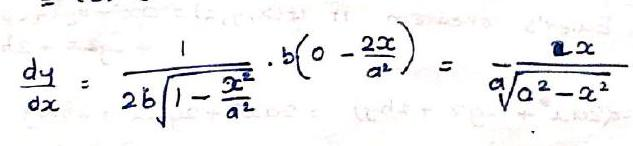
\includegraphics[max width=\textwidth]{2024_07_21_60638e05521ca5966d28g-2}
\end{center}

$$
\begin{aligned}
& \therefore \frac{d u}{d x}=\cos \left(x^{2}+y^{2}\right) \cdot\left(2 x-\frac{2 x y}{a \sqrt{a^{2}-x^{2}}}\right)
\end{aligned}
$$

$$
\text { 2) } \frac{d u}{d x}=
$$

\section*{Euler's Theorem}
let $f(x, y)$ be a homogeneous function of degree ' $n$ ' then "euler's theorem:

$$
x \cdot \frac{\partial f}{\partial x}+y \cdot \frac{\partial f}{\partial y}=n \cdot f \quad \text { or } \sum_{i \in y} i \frac{\partial f}{\partial i}=n \cdot f
$$

\section*{Proof}
$$
\begin{aligned}
\text { Let } u & =x^{n} f(y / x) \\
\therefore \frac{\partial u}{\partial x} & =x^{n} f^{\prime}(y / x) \cdot \frac{-y}{x^{2}}+n x^{n-1} f\left(\frac{y}{x}\right) \\
x \cdot \frac{\partial u}{\partial x} & =-x^{n-1} y f^{\prime}\left(\frac{y}{x}\right)+n x^{n} f\left(\frac{y}{x}\right) \\
\frac{\partial u}{\partial y} & =x^{n} f^{\prime}\left(\frac{y}{x}\right) \cdot \frac{1}{x}+0 \\
y \cdot \frac{\partial u}{\partial y} & =x^{n-1} f^{\prime}\left(\frac{y}{x}\right) \\
\therefore x \cdot \frac{\partial u}{\partial x}+y \cdot \frac{\partial u}{\partial y} & =n x^{n} f\left(\frac{y}{x}\right)-x^{n-1} y f^{\prime}\left(\frac{y}{x}\right)+x^{n-1} y f^{\prime}\left(\frac{y}{x}\right) \\
& =n \cdot u
\end{aligned}
$$

$\begin{aligned} \text { Verity Euler's theorem if } t(x, y, x)= & a x^{2}+b y^{2}+c z^{2}+2 f y z \\ & +2 a z x+2 b x y\end{aligned}$

$x \cdot \frac{\partial \phi x}{\partial x}=2\left(2 a x^{2}+2 g z+2 h y\right)=2 a x^{2}+2 g x z+2 b x y$

$y \cdot \frac{\partial f}{\partial y}=y(2 b y+2 f z)=2 b y^{2}+2 f y z$

$z \cdot \frac{\partial f}{\partial z}=2(2 c z+2 f y+2 g x)=2 c z^{2}+2 f y z+2 g x z$

$\begin{aligned} \therefore x \cdot \frac{\partial f}{\partial x}+y \cdot \frac{\partial f}{\partial y}+z \cdot \frac{\partial f}{\partial z} & =2 a x^{2}+2 b y^{2}+2 c z^{2}+34 f_{y} z+4 y x z+4 h x y \\ & =2(\ldots)\end{aligned}$ $=2 \cdot 4$

$\therefore$ Euler's theorem is verifred

\begin{enumerate}
  \setcounter{enumi}{1}
  \item If $u=\sin ^{-1}\left((x+2 y+3 z) /\left(x^{8}+y^{8}+z^{8}\right)\right)$, find $x \cdot \frac{\partial y}{\partial x}+y \cdot \frac{\partial y}{\partial y}+z \cdot \frac{\partial y}{\partial z}$. $u=\sin ^{-1}\left(\frac{x+2 y+3 z}{x^{8}+y^{8}+z^{8}}\right)$
\end{enumerate}

This is not homogeneous functoon. To malce it

homogeneous, take $\sin \theta$.

$\cos \sin (4)=\frac{x+2 y+3 x}{x^{8}+y^{8}+z^{8}} \equiv \frac{x \cdot\left(1+\frac{2 y}{x}+\frac{3 z}{x}\right)}{x^{8}\left(1+\left(\frac{y}{x}\right)^{8}+\left(\frac{z}{3 c^{2}}\right)\right.}$

$$
\equiv \underbrace{x^{-7}}_{\text {degrec }=-7} \cdot f\left(\frac{y z}{x}\right)
$$

By Euler's theorem: $x \cdot \frac{\partial \omega}{\partial x}+y \cdot \frac{\partial \omega}{\partial y}+z \cdot \frac{\partial \omega}{\partial x}=-7 \cdot \omega$

$\Rightarrow x \cdot \cos (\omega) \cdot \frac{\partial u}{\partial x}+y \cdot \cos (u) \frac{\partial u}{\partial y}+z \cdot \cos (u) \cdot \frac{\partial u}{\partial z}=-7 \cdot \sin (\omega)$

$\Rightarrow x \frac{\partial u}{\partial x}+y \cdot \frac{\partial u}{\partial y}+z \cdot \frac{\partial u}{\partial z}=-7 \frac{\sin (u)}{\cos (u)}=-7 \tan (u)$

$$
=-7 \cdot \tan \left(\sin ^{-1}\left(\frac{x+2 y+3 z}{x^{3}+y^{8}+z^{8}}\right)\right)
$$

verify Euler's theorem, if $u=\sin ^{-1}((x+y) /(\sqrt{x}+\sqrt{y}))$ Hence find $x \partial u / \partial x+2 g . \partial u / \partial y$

$$
u=\sin ^{-1}\left(\frac{x+y}{\sqrt{x}+\sqrt{y}}\right) \Rightarrow \sin (u)=\frac{x+y}{\sqrt{x}+\sqrt{y}} \equiv x^{v_{2}} \times \frac{1+\frac{y}{x}}{1+\sqrt{y}}
$$

let $\varepsilon=\sin (u), \therefore$ By Euler's theorem

$x \cdot \frac{\partial \xi}{\partial x}+y \cdot \frac{\partial \varepsilon}{\partial y}+q \cdot \frac{\partial \xi}{\partial z}=\cos (u)\left[x \cdot \frac{\partial u}{\partial x}+y \cdot \frac{\partial u}{\partial y}+\frac{\partial y}{\partial x}\right]=\frac{1}{2} \sin (\omega)$ $\therefore x \cdot \frac{\partial y}{\partial x}+y \cdot \frac{\partial y}{\partial y}=\frac{1}{2} \tan (u)=\frac{1}{2} \tan \left(\sin ^{-1}\left(\frac{x+y}{\sqrt{x}+\sqrt{y}}\right)\right)$ $u=\sin ^{-1}(\ldots) \Longrightarrow u=\sin ^{-1}\left(\sqrt{x}-\sqrt{y} \quad \frac{1}{\sqrt{1-y^{2}}}\right.$

\begin{center}
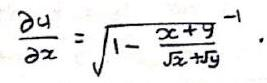
\includegraphics[max width=\textwidth]{2024_07_21_60638e05521ca5966d28g-3}
\end{center}

\section*{Kf Zet $=$}
$$
\begin{aligned}
& \text { If } u=\log \left[\left(x^{4}+y^{4}\right) /(x+y)\right], \text { find } x \cdot \frac{\partial u}{\partial x}+y \cdot \frac{\partial u}{\partial y} \\
& \begin{aligned}
& \text { let } x=e^{u}= \frac{x^{4}+y^{4}}{x+y} \equiv x^{3} \cdot \frac{1+\left(\frac{y}{x}\right)^{4}}{1+y / x} \quad \therefore \text { deg:3 } \\
& \therefore \text { By Euleriss theorem: } x \cdot \frac{\partial x}{\partial x}+y \cdot \frac{\partial x}{\partial y}=3 \cdot x \\
&=x \cdot e^{4} \cdot \frac{\partial u}{\partial x}+y \cdot e^{4} \cdot \frac{\partial u}{\partial y}=3 \cdot e^{u} \\
& \Rightarrow x \cdot e \frac{\partial u}{\partial x}+y \cdot \frac{\partial u}{\partial y}=3
\end{aligned}
\end{aligned}
$$

\section*{Errors \& approximations}
If $\delta x$ and $\delta y$ represents small increments is $x$ and $y$ then our new function is:

$$
f(x+\delta x, y+\delta y)
$$

Hence exparding $f(x+\delta x \neq y+\delta y)$ by Taylor's series by supp supposing $\delta x$ and $\delta y$ be small, so othat their products, squares and higher powers can be neglected then, the error in the function clenoted os $\delta f$ is $\delta f=\frac{\partial f}{\partial x} \delta x+\frac{\partial f}{\partial y} \delta y$.

*: If $\delta y$ is error made in calculating $y$, the relative error in $y$ represented by:

$\frac{\delta y}{y}$

percentage error in $y: \frac{\delta y}{y} \times 100$

Radius of a sphere is found to be 10 cm , with a possible error of 0.2 cm , what is the relative error in the computed volume

A) $r=10 \mathrm{~cm}, \delta r=0.2$

Volume ( $v$ ) $=\frac{4}{3} \pi r^{3}$

error in computing volume: $\delta V=\frac{\partial V}{\partial F} \cdot \delta \gamma$

$$
\begin{aligned}
& =4 \pi r^{2} .8 r \\
& =4 \pi \times 10^{2} \times 0.2 \\
& =251.3 \mathrm{~cm}^{3}
\end{aligned}
$$

volume $(r=40), v=\frac{4}{3} \pi r^{3}=4188.8 \mathrm{~cm}^{3}$

$\therefore$ Be

$\therefore$ Relotive error: $\frac{\delta V}{V}=\frac{251.3}{4188.8}=0.060$

\begin{enumerate}
  \setcounter{enumi}{1}
  \item The diameter and altitude of a can in the spope of a right circular cylinders measured as $4 \mathrm{~cm} \& 6 \mathrm{~cm}$ respectively. The possible error in eoch measurement is 0.1 cm find approximately the maximum possible errov in the volue computed for volume and loteral surface area
\end{enumerate}

$$
\begin{aligned}
& \text { volume }=\pi\left(\frac{D}{2}\right)^2 \cdot h=V=\frac{\pi}{4} D^2 \cdot h \\
& \therefore \partial \delta v=\frac{\partial v}{\partial D} \delta D+\frac{\partial V}{\partial h} \cdot \delta h \quad \text { (approx.) } \\
& =\frac{\pi}{2} D \cdot L \cdot \delta D+\frac{\pi}{4} D^2 \cdot \delta h \\
& =\frac{\pi}{20}\left(4 \times 6+4^2\right)=2 \pi \\
& L S A=\pi D K, 2: S \\
& \therefore \delta S=\frac{\partial S}{\partial D} \cdot \delta D+\frac{\partial S}{\partial h} \cdot \delta h \quad \text { (approx) } \\
& =\pi \times 0.1(h+0) \\
& =\pi \mathrm{cm}^2 \text { (approx). } \\
&
\end{aligned}
$$
3. The focal length of mirror is given by the formula:
$$
\frac{2}{f}=\frac{1}{v}-\frac{1}{u}
$$

If equal errors $k$ are made in the determination of $u$ and $v$, sow that the relative error in the $f$ is given by: $k \cdot\left(\frac{1}{v}+\frac{1}{u}\right)$

$$
\begin{aligned}
& \frac{2}{f}=\frac{1}{v}-\frac{1}{u} \\
& \therefore f=2 \cdot \frac{u v}{u-v} \equiv 2\left(\frac{1}{v}-\frac{1}{u}\right)^{-1} \\
& \delta f=\frac{\partial f}{\partial u} \delta u+\frac{\partial f}{\partial v} \cdot \delta v \\
& =k\left(\frac{\partial f}{\partial u}+\frac{\partial f}{\partial v}\right) \\
& =2 k \cdot\left(-\left(\frac{1}{v}-\frac{1}{u}\right)^{-2}\left(+\frac{1}{u^2}\right) \quad-\left(\frac{1}{v}-\frac{1}{4}\right)^{2^2}\left(-\frac{1}{v^2}\right)\right) \\
& \therefore \frac{\delta f}{f}=\frac{1}{v}\left(-\left(\frac{1}{v}-\frac{1}{u}\right)^{-1} \cdot \frac{1}{u^2}+\left(\frac{1}{v}-\frac{1}{u}\right)^{-1} \frac{1}{v^2}\right) \\
& =\sin \left(-\frac{u^v}{u^2} \cdot \frac{1}{u^2}+\frac{u v}{u-v} \cdot \frac{1}{v^2}\right) \\
& =\left\{\frac{u^2-v^2}{(u v)^2} \cdot \frac{u v}{u-v}\right\} \\
& \left.=\text { k. \{ } \frac{u+v}{u v}\right\} \\
& \frac{\delta f}{\delta}=b_r k \cdot\left(\frac{1}{u}+\frac{1}{v}\right) \\
& \frac{2}{5}=\frac{1}{2}-\frac{1}{4} \\
& -\frac{2}{f^2} \delta f=-\frac{1}{v^2} \delta v+\frac{1}{u^2} \delta u \\
&
\end{aligned}
$$

4. If the I HP required to propel a steamer varies os the cube of the velocity and square of its length, prove that a $3 \%$ increase in velocity and $5 \%$ increase in length will require, an increase of about $17 \%$ in HP.
A)
$$
\begin{aligned}
& H=k \cdot v^3 \cdot v^2 . \\
& \delta v A=0.03 \delta 2 / 2=0.04 \\
& \frac{\delta H}{H}=\frac{k \cdot 3 v^2 \cdot 2^2 \delta v+k \cdot 2 v^3 2 \delta 2}{k \cdot v^3 \eta^2} \quad 3 \frac{\delta v}{V}+2 \frac{\delta 2}{82}=3 \times 0.03+2 \times 0.4=0 \Leftrightarrow
\end{aligned}
$$

Coordinate Systems
$G(x, y, z) \mapsto S(x, \theta, y), \gamma=\sqrt{x^{2}+y^{2}+z^{2}}$

\begin{center}
% \includegraphics[max width=\textwidth]{2024_07_21_847e2aab63d28cbf0193g-1(2)}
\end{center}

\begin{center}
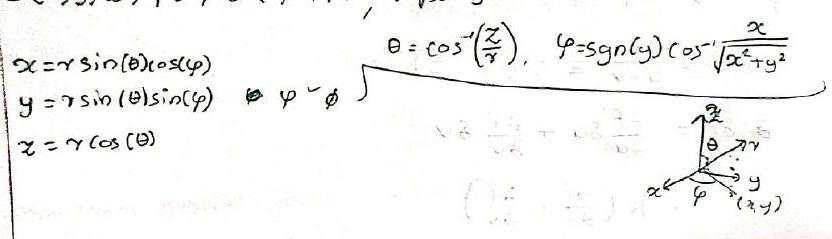
\includegraphics[max width=\textwidth]{2024_07_21_847e2aab63d28cbf0193g-1(1)}
\end{center}

\begin{enumerate}
  \item Relation b/w cortesion and polar co-ordinates:
\end{enumerate}

$(x, y) \mapsto(r \cos (\theta), r \sin (\theta))$, where $\gamma=\sqrt{x^{2}+y^{2}}$

$\theta=\tan ^{-1}$

Here $(x, y)$ changed to $(r, \theta)$

$$
\text { or } J\left(\frac{x, y}{r, \theta}\right)=\gamma
$$

\begin{enumerate}
  \setcounter{enumi}{1}
  \item b/w cortesian and cylindrical co-ordinates:
\end{enumerate}

$$
(x, y, z) \longmapsto(r \cos (\theta), r \sin (\theta), z)
$$

Here $(x, y, z)$ changed to $(r, \theta, z)$

$$
\ldots J\left(\frac{x, y, z}{r, \theta, z}\right)=\gamma
$$

\begin{enumerate}
  \setcounter{enumi}{2}
  \item Cartesian \& spherical coordinates: $[(x, y, z): \rightarrow(x, \phi, \phi)]$
\end{enumerate}

$(x, y, z) \longmapsto(r \sin (\theta) \cos (\phi), r \sin (\theta) \sin (\phi), r \cos (\theta))$ $J\left(\frac{x, y, z}{r, \theta, \phi}\right)=r^{2} \cdot \sin (\theta)$

Convert $x^{2}+y^{2}=4 x$ into polor curve

$x \mapsto r \cos (\theta), y \mapsto r \sin (\theta)$

$$
\gamma^{2}\left(\cos ^{2}(\theta)+\sin ^{2}(\theta)\right)=4 r \cos (\theta)
$$

$$
\text { or } r=4 \cos (\theta)
$$

Express the point: $(x, y, z)=(1,-\sqrt{3}, 2)$ in cylindrical corrdinates

$$
\begin{aligned}
& (x, y, z) \longmapsto(r \cos (\theta) \sim \sin (\theta), z) \\
& \gamma=\sqrt{x^{2}+y^{2}}=\sqrt{1+3}=2 \\
& \theta=\tan ^{-1}\left(\frac{y}{x}\right)=\tan ^{-1}(-\sqrt{3})=-60^{\circ}
\end{aligned}
$$

$$
(x, y, z) \equiv(r, \theta, z) \equiv\left(2,-60^{\circ}, 2\right) \equiv\left(2,-\frac{\pi}{3}, 2\right)
$$

Transform equation in spberical coordinates,

$$
x^{2}+y^{2}+z^{2}=2 z^{2}
$$

$\gamma^{2} \sin ^{2}(\theta) \cos ^{2}(\varphi)$

$$
=(\Delta) \sin ^{2}(\phi)+\gamma^{2} \cos ^{2}(\phi)=2 \gamma^{2} \cos ^{2}(\phi)
$$

\begin{center}
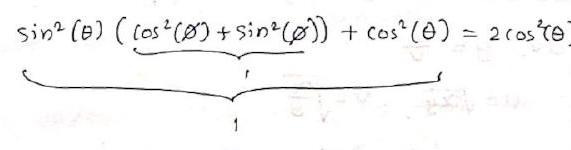
\includegraphics[max width=\textwidth]{2024_07_21_847e2aab63d28cbf0193g-1}
\end{center}

$$
2 \cos ^{2}(\theta)=1
$$

$\theta=\cos ^{-1}\left(\frac{1}{\sqrt{2}}\right)$

$\theta=45^{\circ}$

\section*{Jacubian}
If $u, v$ are functions of $x \& y$ then $\partial \frac{(u, v)}{(x, y)}$ or $J\left(\frac{u, u}{x, y}\right)$ is known as Jacobian

$$
\partial^{x}\left(\frac{u, v}{x, y}\right)=\left|\begin{array}{ll}
\frac{\partial u}{\partial x} & \frac{\partial u}{\partial y} \\
\frac{\partial v}{\partial x} & \frac{\partial v}{\partial y}
\end{array}\right|=\partial \frac{(u, v)}{(x, y)}=\frac{\partial(u, v)}{\partial(x, y)}
$$

If Jacobiar $J$ is $\partial\left(\frac{a, v}{x, y}\right)$, then

$$
\begin{array}{r}
J^{\prime}=2\left(\frac{x, y}{u, v}\right) \\
J^{\prime}=\left|\begin{array}{ll}
\frac{\partial x}{\partial u} & \frac{\partial x}{\partial v} \\
\frac{\partial y}{\partial u} & \frac{\partial y}{\partial v}
\end{array}\right|
\end{array}
$$

and vice-versa

In all coses. $J \cdot J^{\prime}=1$

\section*{Functionally Dependent}
functions $u, u$ are said to be functionally dependent, then $J=0$. And it is functionally independent if $J \neq$ if $x=$ u.v and $y=4 / v$, then prove that $J J^{\prime}=1$ $x=u v, y=\frac{u}{v}$

$\therefore u=\sqrt{x y}, v=\sqrt{\frac{x}{y}}$

$\therefore J=\left|\begin{array}{ll}\frac{\partial u}{\partial x} & \frac{\partial u}{\partial y} \\ \frac{\partial v}{\partial x} & \frac{\partial v}{\partial y}\end{array}\right|=\left|\begin{array}{cc}\frac{\sqrt{y}}{2 \sqrt{x}} & \frac{\sqrt{x}}{2 \sqrt{y}} \\ \frac{1}{2 \sqrt{x y}} & \frac{-\sqrt{x}}{2 y \sqrt{y}}\end{array}\right|$

$\therefore J=-\frac{1}{4 y}-\frac{1}{4 y}=-\frac{1}{2 y}$

$\begin{aligned} \therefore J^{\prime}=\left|\begin{array}{ll}\frac{\partial x}{\partial u} & \frac{\partial x}{\partial v} \\ \frac{\partial y}{\partial u} & \frac{\partial y}{\partial v}\end{array}\right|=\left|\begin{array}{cc}v & u \\ \frac{1}{v} & \frac{-u}{v^{2}}\end{array}\right|=-\frac{u}{v}-\frac{u}{v} & =-2 \frac{u}{v} \\ & =-2 \frac{\sqrt{x y}}{\sqrt{x / y}} \\ & =-2 \cdot \sqrt{x} \cdot \sqrt{y} \cdot \frac{\sqrt{y}}{\sqrt{x}}\end{aligned}$

\section*{$\therefore J \cdot J^{\prime}=-\frac{1}{2 y} x-2 y=1$}
\begin{itemize}
  \item If $r t-s^{2}<0$. neither minimum nor maximum exists - If $r t-s^{2}=0$, Further verification is needed.
\end{itemize}

\section*{Langrangis methud}
For finding max/min of 3 or more variables find $\max / \mathrm{min}$ of $f$, wrtconitruint Working rule

\begin{itemize}
  \item let $F=f(x, y, z)+\lambda \dot{\phi}(x, y, z)$
  \item Simplifying equations: $\frac{\partial F}{\partial x}=0, \frac{\partial F}{\partial y}=0, \frac{\partial F}{\partial z}=0$ we get $\times$ rel.blw. $x, y, z$ and substituting in any of equation, we get their values
\end{itemize}

Examine following functions for extreme value\\
a) $f(x, y)=x^{4}+y^{4}+4 x y-2 x^{2}-2 y^{2}$

$f(x, y) \rightarrow \lambda \beta(x, y)$

A)

$\frac{\partial f}{\partial x}=4 x^{3}+4 y-4 x, \quad \frac{\partial f}{\partial y}=4 y^{3}+4 x-4 y^{2}$

let $\frac{\partial f}{\partial x}=0 \Rightarrow 4 x^{3}+4 y-4 x=0 \Rightarrow y=x-x^{3}$-1 $\frac{\partial f}{\partial y}=0 \Rightarrow 4 y^{3}+4 x-4 y=0 \Rightarrow x=y-y^{3}$-(2)

let $r=\frac{\partial^{2} f}{\partial x^{2}}=12 x^{2}-4$

$$
s=\frac{\partial^{2} f}{\partial x \partial y}=4
$$

$t=\frac{\partial^{2} f}{\partial y^{2}}=12 y^{2}-4$

$\therefore 7+-5^{2}=\left(12 x^{2}-4\right)\left(12 y^{2}-4\right)-16$

$(1)+(2): \quad-y^{3}-x^{3}+x+y=x+y$

$$
\Rightarrow x^{3}+y^{3}=0 \quad \Rightarrow \quad x=-y
$$

Substiture these in $\operatorname{\omega }$ :

$$
-x=x-x^{3} \Rightarrow x^{2}=2 x \Rightarrow x=+\sqrt{2}
$$

substitute in (2):

$$
-y=y-y^{3} \Rightarrow y= \pm \sqrt{2}
$$

for $x= \pm \sqrt{2}, y= \pm \sqrt{2}, \quad \gamma t-s^{2}=384$

to

$\therefore r+-5^{2}>0$

$r=20>0$

$\therefore$ minima exists at $x= \pm \sqrt{2}, y= \pm \sqrt{2}$

$\therefore$ minimum value is $\quad+( \pm \sqrt{2}, \pm \sqrt{2})=8-8$

\section*{b) $f\left(x \in x^{5}-5 x^{4}+5 x^{3}-1\right.$}
\begin{enumerate}
  \setcounter{enumi}{1}
  \item A rectangular box open at the top is to have the volume $32 \mathrm{ft}^{3}$. find dimensions of box requiring least amount of material for its construd $v=x y z=32 \mathrm{ft}^{3}$
\end{enumerate}

$L S A:=A=x y+2 x z+2 y z$

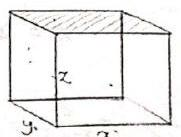
\includegraphics[max width=\textwidth, center]{2024_07_21_847e2aab63d28cbf0193g-2}\\
tet $E=v$

\begin{center}
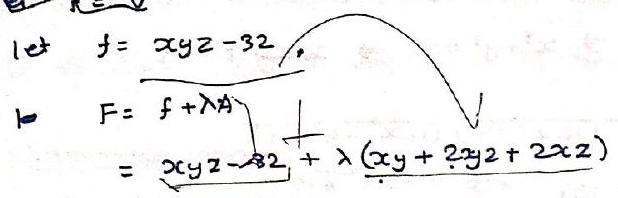
\includegraphics[max width=\textwidth]{2024_07_21_847e2aab63d28cbf0193g-3(2)}
\end{center}

$\frac{\partial F}{\partial x}=0 \Rightarrow y z+\lambda(y+2 z)=0-10 \frac{\partial F}{\partial z}=0 \Rightarrow x y+\lambda(2 y+2 x)=0$

$\frac{\partial F}{\partial y}=0 \Rightarrow x z+\lambda(x+2 z)=0-2$

\#

x. (1) $x-$ (2) $y::$

$\Rightarrow 2 \times 2(x-y)=0 \quad \Rightarrow \longrightarrow \underset{\rightarrow y=0}{\rightarrow} y$

(2). $y$-(9) $z$

$\Rightarrow \lambda(x y+z z z y-2 y z-z z)=0$

\begin{center}
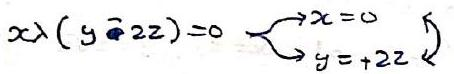
\includegraphics[max width=\textwidth]{2024_07_21_847e2aab63d28cbf0193g-3(1)}
\end{center}

$\therefore x=y, y=2 z, z=y / 2$

\section*{Substitute in $x_{y} z=32$}
$$
\begin{aligned}
& \therefore 32=y \cdot y \cdot y / 2 \Rightarrow y=64 \Rightarrow y=24 \\
& 32=x \cdot x: x / 2 \Rightarrow x=4 \\
& 32=2 z \cdot 2 z: z \Rightarrow 2=2
\end{aligned}
$$

3 find max \& min of points, $A(3,4,12)$ from the sphere $x^{2}+y^{2}+z^{2}=1$

A) Llet $P=(a, b, c)$ on point closest tuA. $\therefore P=(x 3, \lambda 4,>12)$

\begin{center}
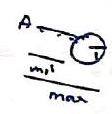
\includegraphics[max width=\textwidth]{2024_07_21_847e2aab63d28cbf0193g-3}
\end{center}

$\therefore|P|=1 \Rightarrow 9 \lambda^{2}+16 \lambda^{2}+144 \lambda^{2}=1 \Rightarrow$ $169 \lambda^{2}=1 \Rightarrow \lambda=1 / 13$

$\therefore=\left(\frac{3}{13}, \frac{4}{13}, \frac{12}{13}\right)$

$\therefore$ min. distance $=\sqrt{\left(3-\frac{3}{13}\right)^{2}+\left(4-\frac{4}{13}\right)^{2}+\left(12-\frac{12}{13}\right)^{2}}$

$$
=\underline{\underline{12}}
$$

$\therefore$ max distance on is to point on opposite side $=12+2=1$ sunnts

let $p$ be a point on sphore $P=(x, y, z)$

$\therefore \operatorname{dist}(A, P)^{2}=(3-x)^{2}+(4-y)^{2}+(12-2)^{2}=D$ $\frac{\partial F}{\partial y}=0 \Rightarrow$

$\partial y=0 \Rightarrow-2(4-y)+2 x y=0 \Rightarrow y=\frac{4}{\lambda-1}$

$\frac{\partial F}{\partial z}=0 \Rightarrow-2(12-2)+2 z=0 \Rightarrow z=\frac{12}{\lambda-1}$

$$
\therefore \quad x^{2}+y^{2}+z^{2}=1
$$

$$
\Rightarrow \frac{1}{\left(\lambda^{2}-1\right)^{2}}(9+16+144)=1
$$

\section*{$\lambda-1= \pm 13 \Rightarrow \lambda=-12$ or 19}
for $\lambda=12$

$x=\frac{-3}{-13}, y=\frac{4}{-13}, z=\frac{12}{-13}$

$\lambda=14 \quad x=\frac{3}{13}, y=\frac{4}{13}, z=\frac{12}{13}$

let $P=\left(\frac{3}{13}, \frac{4}{13}, \frac{12}{13}\right), Q=\left(\frac{-3}{13},-\frac{4}{13},-\frac{12}{13}\right)$

$\begin{aligned} \therefore A P & =\sqrt{\left(3-\frac{3}{13}\right)^{2}+\left(4-\frac{4}{13}\right)^{2}+\left(\frac{12}{13}-12\right)^{2}}=12 \\ A Q & =\sqrt{\left(3+\frac{3}{13}\right)^{2}+\left(4+\frac{4}{13}\right)^{2}+\left(12+\frac{12}{13}\right)^{2}}=14\end{aligned}$

$\therefore$ minimum distance $=12, \max =14$

\begin{enumerate}
  \setcounter{enumi}{3}
  \item Find shortest distance from the origin to byporbolu
\end{enumerate}

$x^{2}+8 x y+7 y^{2}=225$

A) let $P(x, y)$ be a point on byperbola.

distance from $0 \rightarrow P=D=\sqrt{x^{2}+y^{2}}$

$$
D^{2}=x^{2}+y^{2}
$$

let $F=D^{2}+\lambda\left(x^{2}+8 x y+7 y^{2}-225\right)$.

$$
\begin{aligned}
& \frac{\partial F}{\partial x}=2 x+\lambda(2 x+8 y)=0-(1) \\
& \frac{\partial F}{\partial y}=2 y+\lambda(14 y+8 x)=0 \text {-(2) }
\end{aligned}
$$

let $F=D+x\left(x^{2}+y^{2}+z^{2}-1\right)$
    $\therefore \frac{\partial F}{\partial x}=0 \Rightarrow-2(3-x)+x x=0 \Rightarrow x=\frac{6}{2 \lambda-2}=\frac{3}{\lambda-1}$

$$
\begin{array}{ll}
x+\lambda(x+4 y)=0-11 & \Rightarrow(1+\lambda) x+4 \lambda y=0 \\
y+\lambda(7 y+4 x)=0-(2) & \Rightarrow(1+7 \lambda) y+4 \lambda x=0
\end{array}
$$

(3) $x y$

$$
\begin{aligned}
& (1+\lambda) x y+4 \lambda y^{2}=0 \quad-(0) \quad \text { (6) (7) : } \\
& \text { (4) } \times x \cdot(1+7 \lambda) x y+4 \lambda x^{2}=0-(6) \\
& (1+\lambda-1-7 \lambda) x y+4 \lambda\left(y^{2}-x^{2}\right)=0 \\
& (-6 \lambda) x y+4 \lambda\left(y^{2}-x^{2}\right)=0
\end{aligned}
$$


\end{document}